% Chapter Template

\chapter{Diagrammatic notation} % Main chapter title

\label{Chapter3} % Change X to a consecutive number; for referencing this chapter elsewhere, use \ref{ChapterX}

\lhead{Chapter 4. \emph{Diagrammatic notation}} % Change X to a consecutive number; this is for the header on each page - perhaps a shortened title

%----------------------------------------------------------------------------------------
%	Diagrammatic notation
%----------------------------------------------------------------------------------------

\section{Diagrammatic notation - background}

While second quantization provides us with the foundation for working
out expressions within the various many-body methods, it may prove
cumbersome to derive comprehensive equations such as the coupled
cluster equations using only second quantized operators and Wick's
generalized theorem. To this end, the \emph{diagrammatic notation},
originally introduced in the context of  quantum electrodynamics by Richard Feynman
in 1959 \cite[p.1]{ShavittBartlett2009}, will simplify calculations
considerably. In addition, diagrams allow us to easily
identify features of terms in the equations such as which terms vanish
or should be naturally grouped together \cite{ShavittBartlett2009}.

\section{The Slater Determinant}

Due to their origin in quantum field theory, diagrams normally express
a time-ordered sequence of operators where time evolves in the upwards
direction. This might seem strange when applied to the
time-independent Schrödinger equation, but we shall only interpret the
time axis as the sequence in which the different operators are
applied. A starting point for the calculations will be the Fermi
vacuum, expressed simply by a blank space. As we have already shown
(see for example Eqn. \ref{eqn:hamiltonian_N}, normal ordering of the Hamiltonian with respect to the Fermi
vacuum will allow us mainly focus on excited states (represented by
Slater determinants in our representation). These states, or Slater determinants, may be
expressed simply by vertical lines, assigned either upwards- or
downwards arrows to indicate particle or holes, respectively, as in
Figs.~\ref{fig:diag_psi_ai} or \ref{fig:diag_psi_aibj}.
\begin{figure}[p]
    \centering
    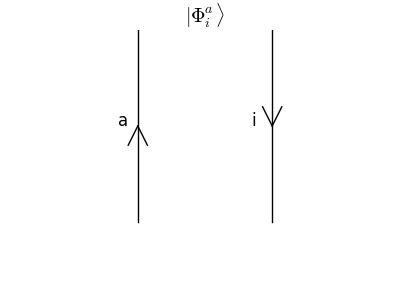
\includegraphics[width=0.5\textwidth]{diag_psi_ai}
    \caption{A Slater determinant with one hole state and one particle state.}
    \label{fig:diag_psi_ai}
\end{figure}

\begin{figure}[p]
    \centering
    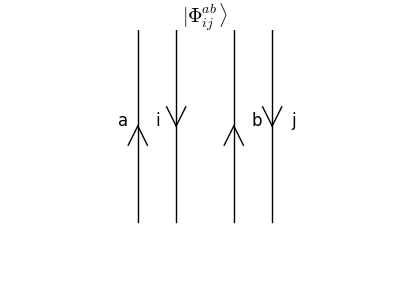
\includegraphics[width=0.5\textwidth]{diag_psi_aibj}
    \caption{A Slater determinant with two hole states and two particle states.}
    \label{fig:diag_psi_aibj}
\end{figure}

\FloatBarrier

\section{Operators}

We will use horizontal dashed lines to represent operators such as
terms in the normal-ordered hamiltonian. While the one-body operator
will have two lines entering and/or leaving, the two-body operator
will have four lines entering and/or leaving. The lines entering from
below represent the annihilation of pseudo particles, while lines
exiting above represent creation of pseudo particles. Following this
logic, we list the normal ordered one-body operator  of Eq.~(\ref{eqn:onebody_N}) 
and the normal ordered two-body operator
of Eq.~(\ref{fig:onebody}) diagrammatically, as shown in Figs.~\ref{fig:onebody},
\ref{fig:twobody1} and \ref{fig:twobody2}.
\begin{figure}[p]
    \centering
    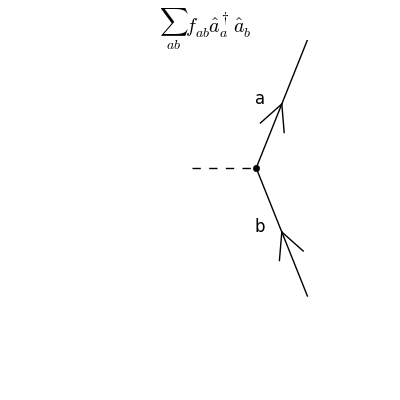
\includegraphics[width=0.4\textwidth]{onebody1}
    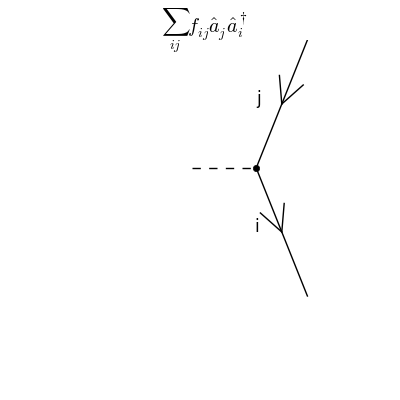
\includegraphics[width=0.4\textwidth]{onebody2}
    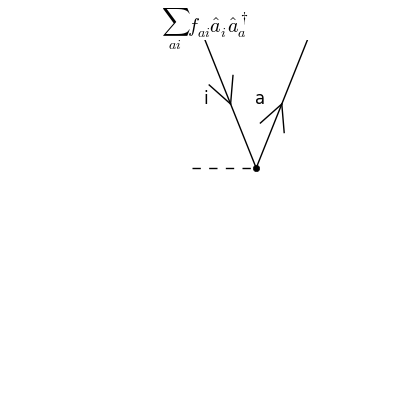
\includegraphics[width=0.4\textwidth]{onebody3}
    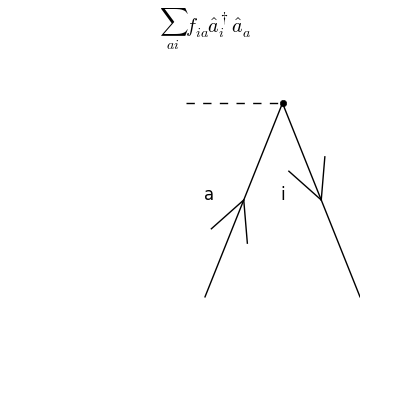
\includegraphics[width=0.4\textwidth]{onebody4}
    \caption{A normal ordered one-body operator with its mathematical expressions.}
    \label{fig:onebody}
\end{figure}

\begin{figure}[p]
    \centering
    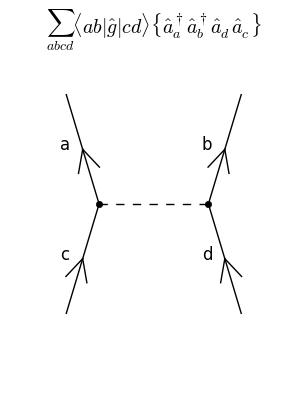
\includegraphics[width=0.4\textwidth]{twobody1}
    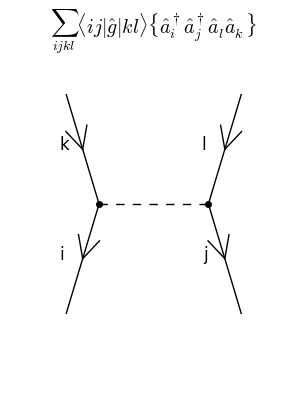
\includegraphics[width=0.4\textwidth]{twobody2}
    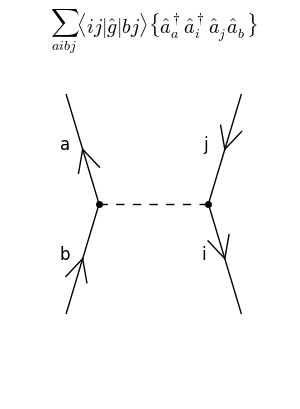
\includegraphics[width=0.4\textwidth]{twobody3}
    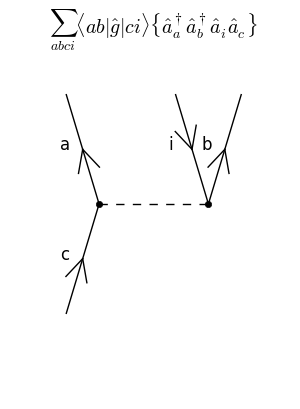
\includegraphics[width=0.4\textwidth]{twobody4}
    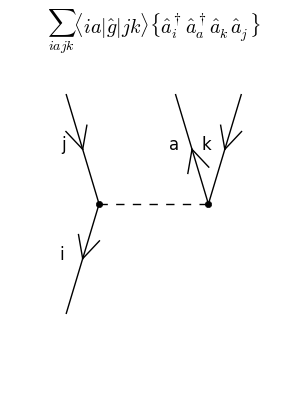
\includegraphics[width=0.4\textwidth]{twobody5}
    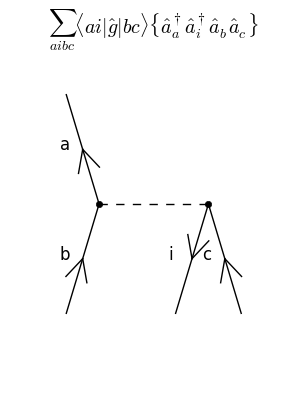
\includegraphics[width=0.4\textwidth]{twobody6}
    \caption{A normal ordered two-body operator with its mathematical expressions.}
    \label{fig:twobody1}
\end{figure}

\begin{figure}[p]
    \centering
    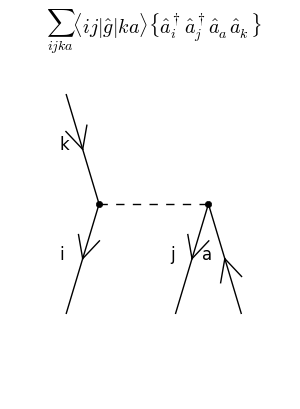
\includegraphics[width=0.4\textwidth]{twobody7}
    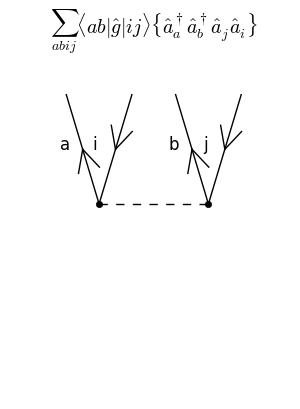
\includegraphics[width=0.4\textwidth]{twobody8}
    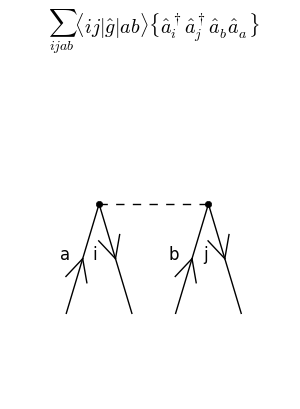
\includegraphics[width=0.4\textwidth]{twobody9}
    \caption{A normal ordered two-body operator with its mathematical expressions (continued).}
    \label{fig:twobody2}
\end{figure}

\FloatBarrier

\section{Contractions}

Diagrams allow us to represent contractions in a straight
forward manner, by connecting lines from Slater determinants to operators or between
operators. For example, we may consider the contraction of a singly
excited Slater determinants with a term in the normal ordered one-body operator, given by 
\begin{equation}
( \sum_{bc} f_{bc} \{  \Cr{b} \An{c} \}) \vert \Phi_i^a \rangle = ( \sum_{bc} f_{bc} \{ \Cr{b} \An{c} \})\{ \Cr{a} \An{i} \} \vert \Phi_0 \rangle = \sum_{bc} f_{bc} \delta_{ac}  \vert \Phi_i^b \rangle,
\label{eqn:onebody_N1}
\end{equation}
where the contraction occurs between the indices in the Kronecker delta, in terms of the  diagrammatic contraction 
performed in Fig. \ref{fig:contraction}.

\begin{figure}[p]
    \centering
    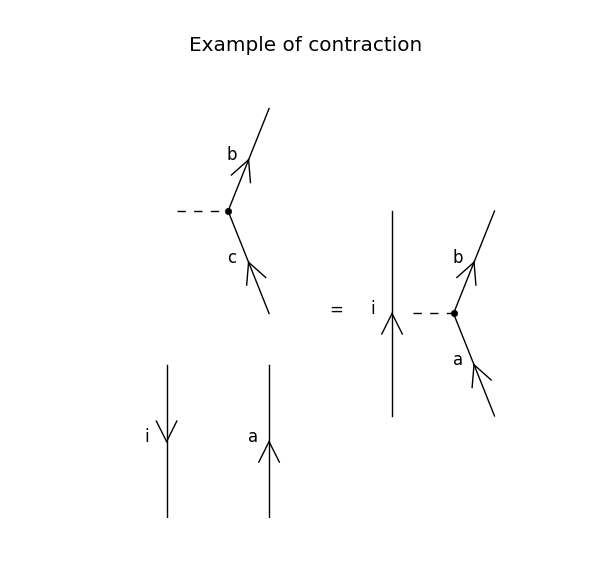
\includegraphics[width=0.7\textwidth]{contraction}
    \caption{A contraction of a one-body operator and a singly excited Slater determinant.}
    \label{fig:contraction}
\end{figure}

The diagrams resulting from this process may in turn be interpreted
back into mathematical expressions that we may use in implementations
of the various many-body methods.


\section{Interpreting diagrams}

The various many body methods which will be introduced in the upcoming
chapters rely on operator expressions and contractions. The basic idea
of using diagrams to derive such expressions may be outlined as
follows. For a given method we shall see that the contracted
expressions that are included in the  evaluation of say the correlation energy, may
be visually represented by a set of diagrams. The situation before
these contractions may also be visually represented by combinations of
such uncontracted vertices as shown in Figs. \ref{fig:twobody1}, \ref{fig:twobody2}, \ref{fig:onebody} (and so on). 

By defining consistent
rules for how the contracted diagrams are obtained from the
uncontracted vertices, we may skip the mathematical contraction
altogether, derive the various resulting terms, and interpret them
back into mathematical expressions by rules that ensure that all
factors and distinct features of the expressions are preserved.

Luckily, such consistent rules are present in the literature
\cite{ShavittBartlett2009} for many of the methods we discuss in the
upcoming chapter.
